\graphicspath{{chapter3/}{manuscript/}}

\begin{center}
\textbf{Unifying individual and metapopulation scales with stochastic
population models: the effect of climate and competition on tree range
limits} \\
Willian~Vieira, Dominique~Gravel
\end{center}

\hypertarget{supplementary-material-1}{%
\subsection{Supplementary Material 1}\label{supplementary-material-1}}

\hypertarget{fig:figsupp1}{%
\begin{figure}
\centering
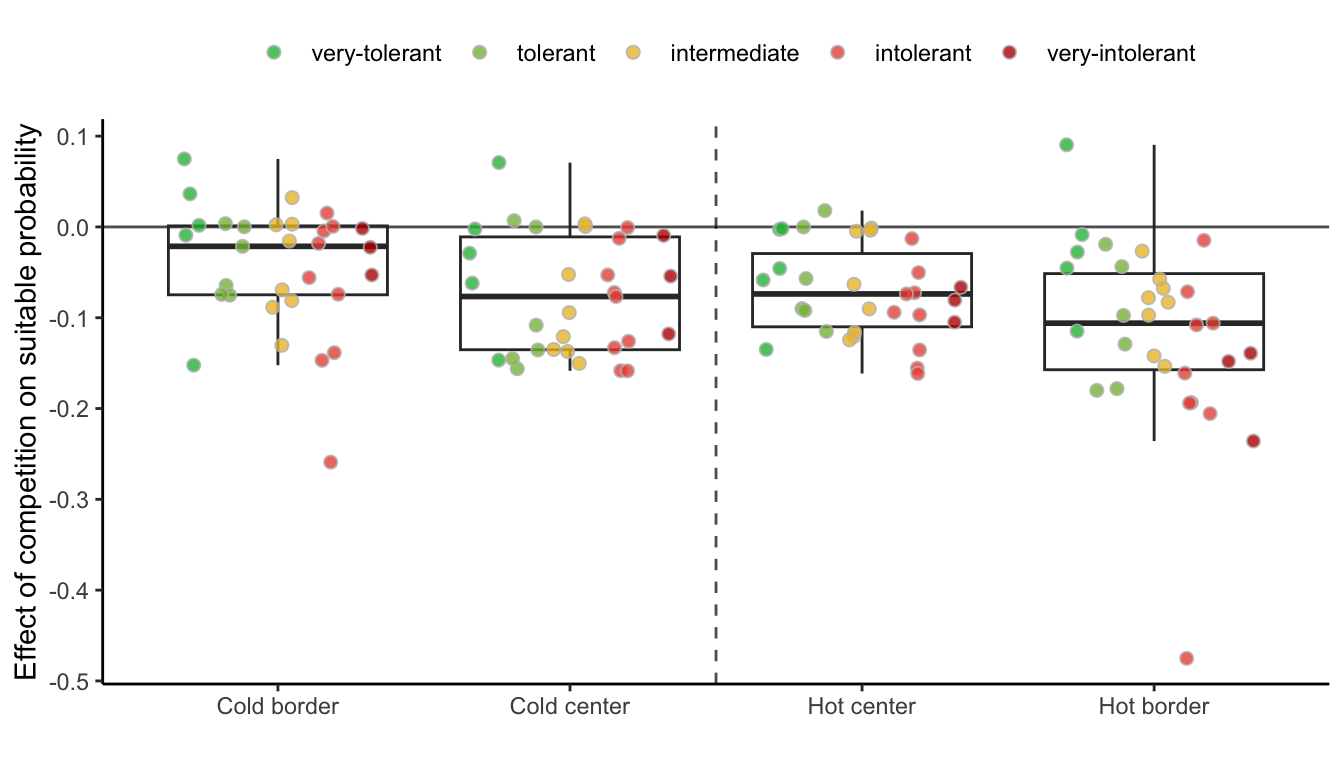
\includegraphics{manuscript/figs/fig-effect_of_comp-1.png}
\caption[{The effect of competition on suitable probability across the
four range positions.}]{The effect of competition on suitable
probability across the four range positions. We assessed the competition
effect by subtracting suitable probability under heterospecific to
suitable probability under no competition. A positive relative
difference indicates an increase in suitable probability from the center
towards the border, while a negative difference indicates a decrease.
Each species point is color-coded based on its shade tolerance following
\citet{burns1990silvics}.}
\label{fig:figsupp1}
\end{figure}
}

\newpage

\hypertarget{fig:figsupp2}{%
\begin{figure}
\centering
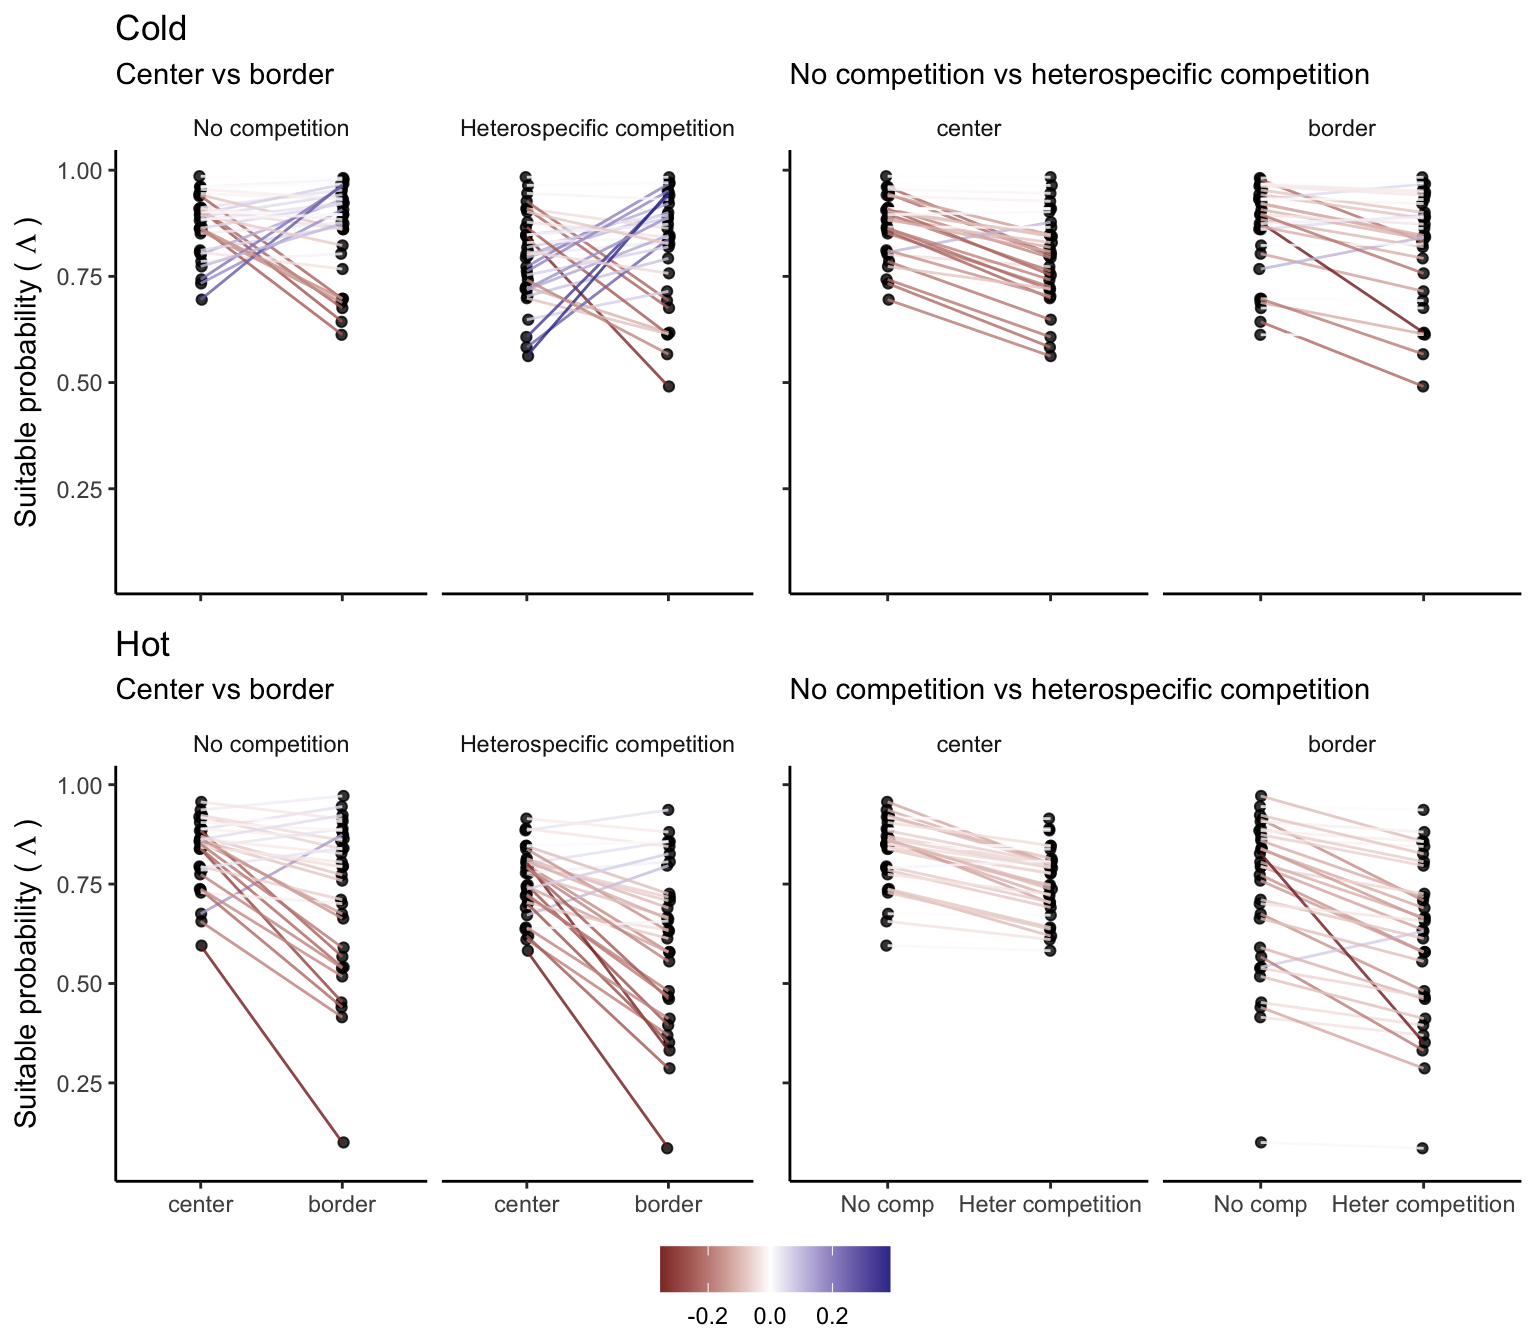
\includegraphics{manuscript/figs/fig-diff_sp_raw-1.png}
\caption[{Difference in suitable probability between the center and
border of the distribution (left panels) and no competition and
heterospecific competition (right) for the cold (top) and hot (bottom)
ranges.}]{Difference in suitable probability between the center and
border of the distribution (left panels) and no competition and
heterospecific competition (right) for the cold (top) and hot (bottom)
ranges. The color of the line connecting each species' conditions
represents the intensity of change in suitable probability---the more
intense the color, the greater the shift between conditions.}
\label{fig:figsupp2}
\end{figure}
}

\newpage

\hypertarget{fig:figsupp3}{%
\begin{figure}
\centering
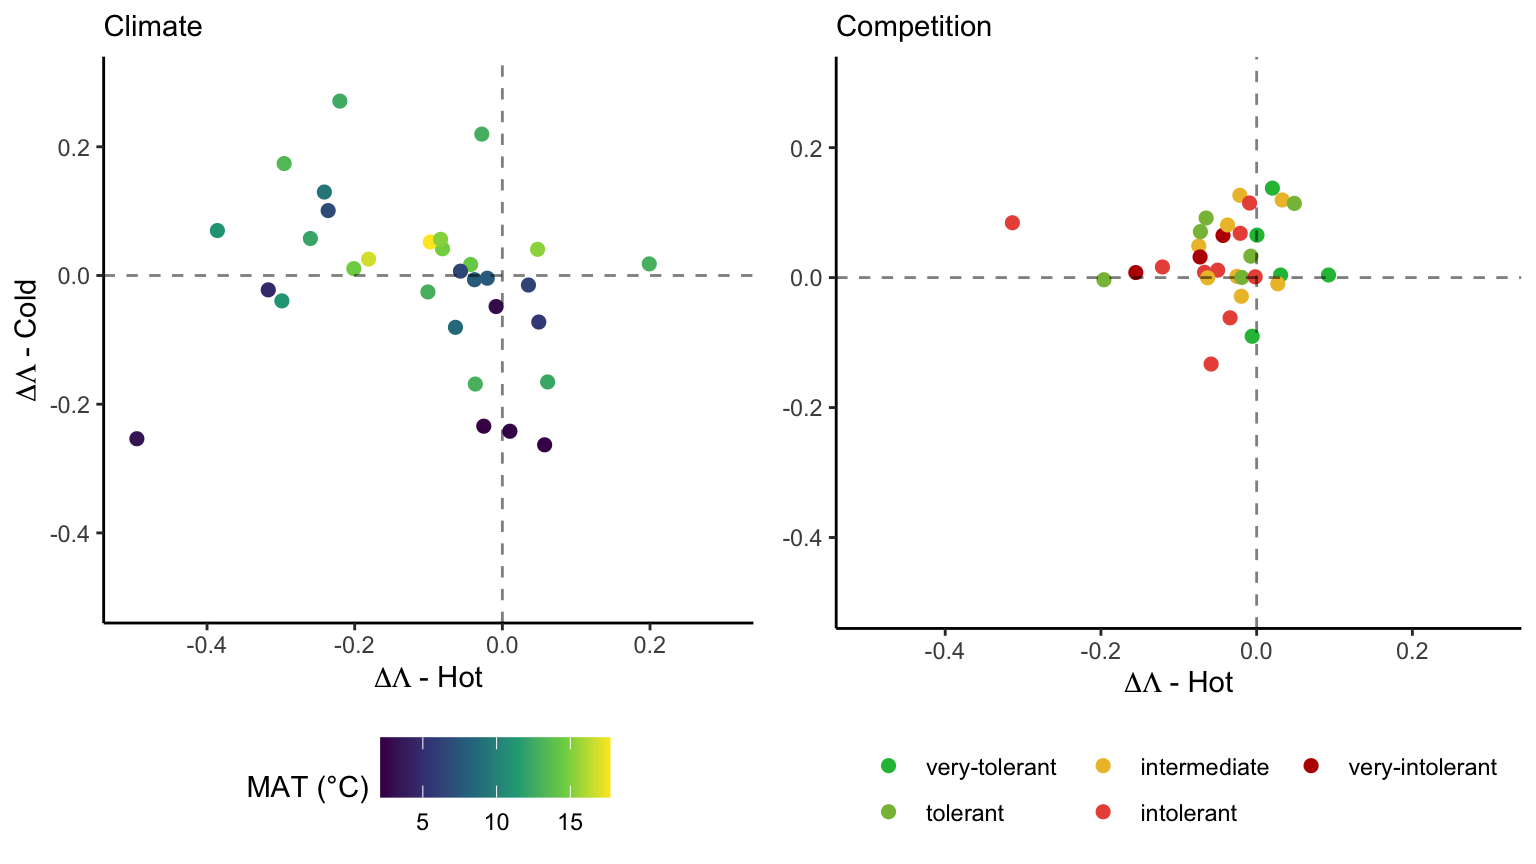
\includegraphics{manuscript/figs/fig-diff_sp_hot_vs_cold-1.png}
\caption[{The relationship in the difference in suitable probability
from the center to the border (\(\Delta\Lambda\)) between the cold and
hot borders.}]{The relationship in the difference in suitable
probability from the center to the border (\(\Delta\Lambda\)) between
the cold and hot borders. A species at the bottom-left area (both
\(\Delta\Lambda\) are negative) indicates an unimodal decrease in
suitable probability at the borders. Conversely, species at the
top-right square exhibit an inverse unimodal shape. In the top-left or
bottom-right areas, suitable probability linearly decreases or increases
from the cold toward the hot border, respectively. For the climate
effect (left panel), species are colored following the centroid mean
annual temperature among all observed plots. In the climate effect (left
panel), species are color-coded based on the centroid of mean annual
temperature among all observed plots. In the competition effect (right
panel), species are classified by shade tolerance following
\citet{burns1990silvics}.}
\label{fig:figsupp3}
\end{figure}
}

\newpage

\hypertarget{fig:figsupp4}{%
\begin{figure}
\centering
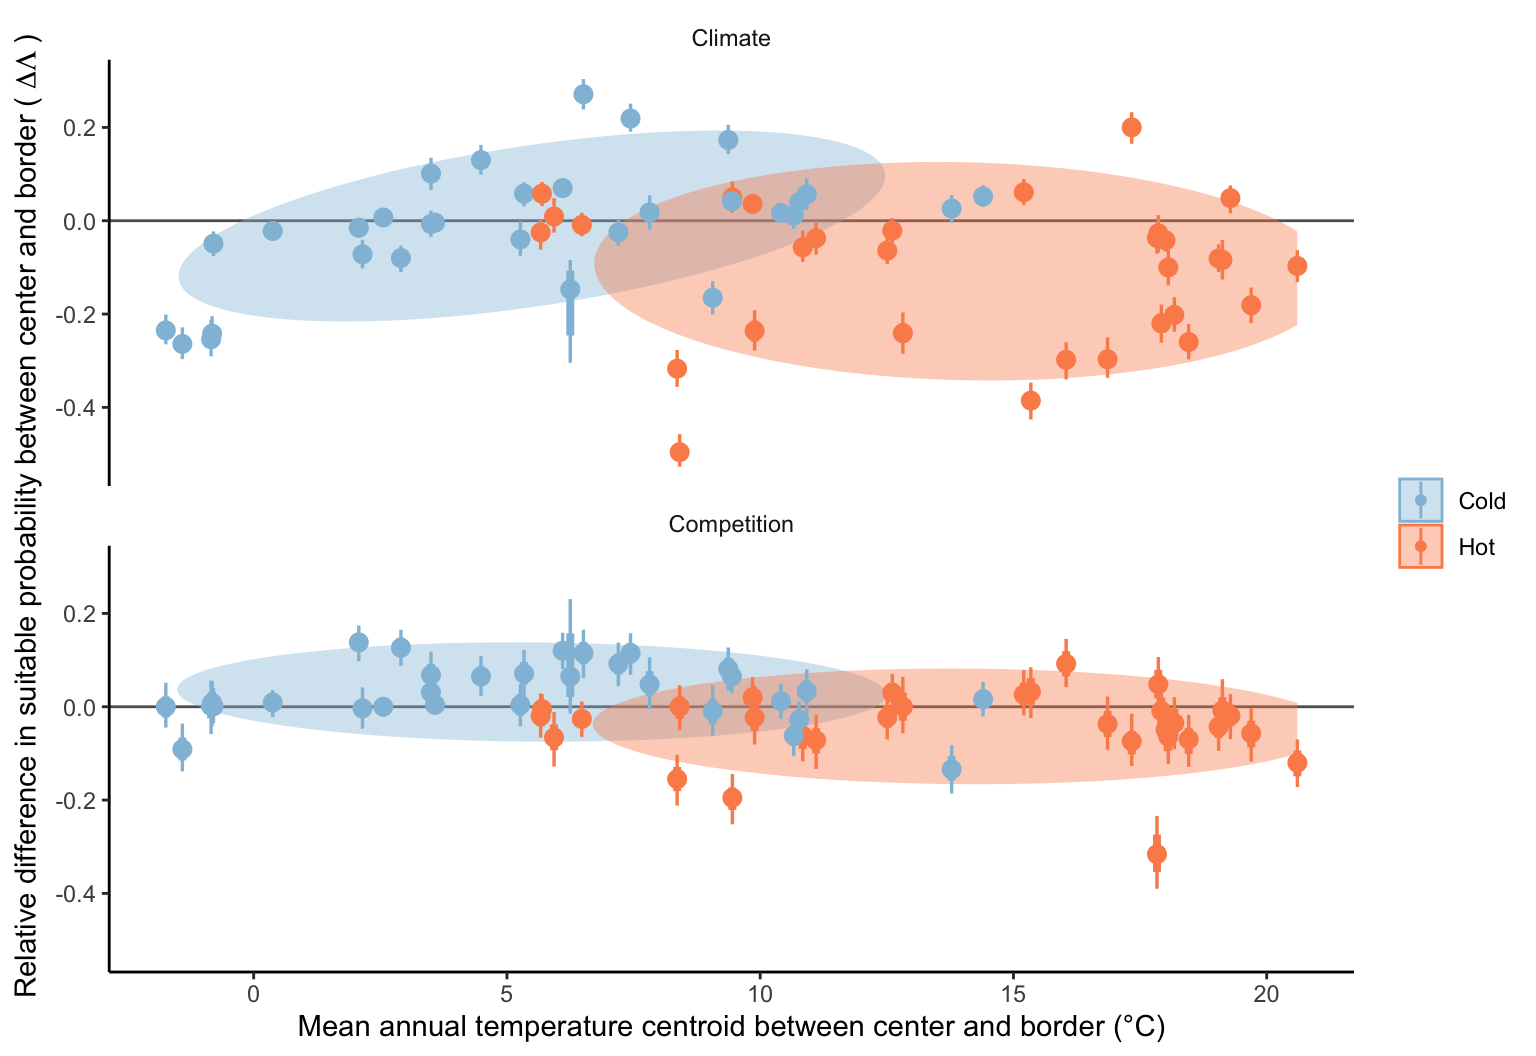
\includegraphics{manuscript/figs/fig-sp_diff_over_MAT-1.png}
\caption[{Relative difference in suitable probability between the center
and border for climate and competition for 31 species located over the
mean annual temperature gradient.}]{Relative difference in suitable
probability between the center and border for climate and competition
for 31 species located over the mean annual temperature gradient.
Species points are grouped by a Multivariate Normal Density function
with 75\% probability.}
\label{fig:figsupp4}
\end{figure}
}

\newpage

\begin{longtable}{lrrr}
\caption{List of species and their frequency across the dataset.}
\label{variability_impl_mech}
\endfirsthead
\endhead
  \toprule
    Species & Number of
    plots & Number of
    individual & Number of
    observation \\
    \midrule\addlinespace[2.5pt]
    \emph{Acer rubrum} & 13149 & 96739 & 235408 \\
    \emph{Abies balsamea} & 11932 & 247737 & 521565 \\
    \emph{Betula papyrifera} & 9508 & 78049 & 203500 \\
    \emph{Picea mariana} & 7869 & 186491 & 454246 \\
    \emph{Acer saccharum} & 7403 & 71961 & 184641 \\
    \emph{Picea glauca} & 5889 & 27641 & 65626 \\
    \emph{Populus tremuloides} & 5876 & 56010 & 127115 \\
    \emph{Betula alleghaniensis} & 5624 & 28872 & 73116 \\
    \emph{Quercus rubra} & 4549 & 18272 & 46341 \\
    \emph{Quercus alba} & 4200 & 20376 & 51466 \\
    \emph{Fagus grandifolia} & 3819 & 21784 & 51764 \\
    \emph{Prunus serotina} & 3730 & 12178 & 26464 \\
    \emph{Thuja occidentalis} & 3230 & 51312 & 125811 \\
    \emph{Pinus strobus} & 3165 & 15638 & 38470 \\
    \emph{Fraxinus americana} & 2885 & 8942 & 21501 \\
    \emph{Quercus velutina} & 2722 & 10068 & 23298 \\
    \emph{Tsuga canadensis} & 2604 & 17914 & 45198 \\
    \emph{Nyssa sylvatica} & 2436 & 6275 & 15785 \\
    \emph{Quercus stellata} & 2279 & 14707 & 32102 \\
    \emph{Picea rubens} & 2190 & 16580 & 41674 \\
    \emph{Liquidambar styraciflua} & 2154 & 11655 & 29671 \\
    \emph{Fraxinus pennsylvanica} & 2149 & 9048 & 20588 \\
    \emph{Tilia americana} & 2059 & 8415 & 21412 \\
    \emph{Pinus banksiana} & 2057 & 34122 & 75372 \\
    \emph{Populus grandidentata} & 2015 & 13759 & 29358 \\
    \emph{Fraxinus nigra} & 1951 & 12633 & 31156 \\
    \emph{Liriodendron tulipifera} & 1912 & 8580 & 21071 \\
    \emph{Carya tomentosa} & 1636 & 3897 & 10590 \\
    \emph{Carya glabra} & 1622 & 4002 & 9916 \\
    \emph{Quercus prinus} & 1590 & 11000 & 27554 \\
    \emph{Juniperus virginiana} & 1571 & 9474 & 21400 \\
  \bottomrule
\end{longtable}

\newpage

\hypertarget{supplementary-material-2}{%
\subsection{Supplementary Material 2}\label{supplementary-material-2}}

The complete figures for the model fit for each species is available in
the following link:
\url{https://willvieira.github.io/book_forest-demography-IPM/extinction_risk.html\#appendices}.

Each figures represents the model fit and the estimation of suitable
probability for the cold and hot ranges for each of the 31 eastern North
American tree species. The model's average line and 90\% prediction
intervals are estimated using 500 draws from the posterior distribution.
The vertical dotted line represents the range limits of the observed
mean annual temperature in the dataset.

\newpage
